%%%%%%%%%%%%%%%%%%%% book.tex %%%%%%%%%%%%%%%%%%%%%%%%%%%%%
%
% sample root file for the chapters of your "monograph"
%
% Use this file as a template for your own input.
%
%%%%%%%%%%%%%%%% Springer-Verlag %%%%%%%%%%%%%%%%%%%%%%%%%%


% RECOMMENDED %%%%%%%%%%%%%%%%%%%%%%%%%%%%%%%%%%%%%%%%%%%%%%%%%%%
\documentclass[pdftex,12pt, oneside]{book}
 
% choose options for [] as required from the list
% in the Reference Guide, Sect. 2.2
%\usepackage[paperwidth=8.5in, paperheight=13in]{geometry} %Folio
\usepackage[paperwidth=8.27in, paperheight=11.69in]{geometry} %A4

\usepackage{makeidx}         % allows index generation
\usepackage{graphicx}        % standard LaTeX graphics tool
                             % when including figure files
\usepackage[bottom]{footmisc}% places footnotes at page bottom
\usepackage[bahasa]{babel}
\usepackage{enumerate}
\usepackage{paralist}
\usepackage{float}
\usepackage{gensymb}  
\usepackage{listings}
\usepackage{color}
\renewcommand{\baselinestretch}{1.5}

\newcommand{\HRule}{\rule{\linewidth}{0.5mm}}

\makeindex             % used for the subject index
                       % please use the style svind.ist with
                       % your makeindex 
                     
\definecolor{codegreen}{rgb}{0,0.6,0}
\definecolor{codegray}{rgb}{0.5,0.5,0.5}
\definecolor{codepurple}{rgb}{0.58,0,0.82}
\definecolor{backcolor}{rgb}{0.95,0.95,0.92}

\lstdefinestyle{mystyle}{
  backgroundcolor=\color{backcolor},
  commentstyle=\color{codegreen},
  keywordstyle=\color{magenta},
  stringstyle=\color{codepurple},
  basicstyle=\footnotesize,
  breakatwhitespace=false,
  breaklines=true,
  captionpos=b,
  keepspaces=true,
  numbers=left,
  numbersep=5pt,
  showspaces=false,
  showstringspaces=false,
  showtabs=false,
  tabsize=2
}

\lstset{style=mystyle}


%%%%%%%%%%%%%%%%%%%%%%%%%%%%%%%%%%%%%%%%%%%%%%%%%%%%%%%%%%%%%%%%%%%%%

\begin{document}
\sloppy


\begin{titlepage}

\begin{center}
{\large DOKUMENTASI RANCANGAN SISTEM BASIS DATA UNTUK SISTEM INFORMASI PEMBAYARAN PAJAK BUMI DAN BANGUNAN PERDESAAN DAN PERKOTAAN DI KABUPATEN BREBES}

\HRule\\[1cm]

PERIODE PENILAIAN TAHUN 2018\\[1cm]


\includegraphics[width=0.5\textwidth]{./resources/logo}\\[1cm]

Oleh :\\
Priyanto Tamami, S.Kom.\\
NIP 19840409 201001 1 025\\


\vfill


Fungsional Pranata Komputer\\
Badan Pengelolaan Pendapatan, Keuangan dan Aset Daerah\\
Pemerintah Daerah Kabupaten Brebes\\
Brebes, 19 Maret 2018
\end{center}

\end{titlepage}

\frontmatter%%%%%%%%%%%%%%%%%%%%%%%%%%%%%%%%%%%%%%%%%%%%%%%%%%%%%%


\begin{center}
{\huge \bfseries Lembar Pengesahan}\\[0.4cm]

\begin{tabular}{l c p{10cm}}
  Nama Kegiatan & : & 	Membuat Petunjuk Operasional Sistem Komputer \\
  Judul & : & PETUNJUK PENGOPERASIAN PROGRAM SISTEM INFORMASI PEMBAYARAN PAJAK BUMI DAN BANGUNAN PERDESAAN DAN PERKOTAAN DI KABUPATEN BREBES \\
\end{tabular}\\[2cm]

\begin{tabular}{c c}
  Disetujui oleh : & Disusun Oleh \\
  Kepala Sub Bidang Keberatan & Pranata Komputer \\
  Pada tanggal 18 April 2018 & Selesai tanggal : 17 April 2018 \\
  & \\
  & \\
  & \\
  M.L. Setiyawan, S.E.Ak & Priyanto Tamami, S.Kom \\
  NIP 19790530 200604 1 006 & NIP 19840409 201001 1 025
\end{tabular}

\end{center}  

\tableofcontents
\listoffigures

\mainmatter%%%%%%%%%%%%%%%%%%%%%%%%%%%%%%%%%%%%%%%%%%%%%%%%%%%%%%%
\chapter{RANCANGAN STRUKTUR BASIS DATA}

Dalam kegiatan pengelolaan Pajak Bumi dan Bangunan sektor Perkotaan dan Perdesaan, Pemerintah Daerah Kabupaten Brebes, dalam hal ini Badan Pengelolaan Pendapatan, Keuangan dan Aset Daerah Kabupaten Brebes menggunakan sistem informasi atau aplikasi yang telah digunakan sebelumnya pada Direktorat Jendral Pajak Kementerian Keuangan Republik Indonesia, yaitu aplikasi SISMIOP (Sistem Manajemen Informasi Objek Pajak).

Dari awal pendataan, penilaian, penetapan, penagihan, pelaporan dan pencatatan pembayaran seluruhnya sudah dapat diakomodir oleh SISMIOP ini. Bahkan untuk proses Pengurangan atau Keberatan dapat dilakukan oleh aplikasi SISMIOP ini.

Dengan lingkup cakupan aplikasi yang begitu luas, tentunya tidak perlu ada yang ditambahkan lagi, hanya memerlukan beberapa penyesuaian saja. Keterbatasan yang ada pada aplikasi ini adalah berbasis \textit{desktop} dan bergantung dengan Oracle Form 6i. Hal inilah yang menjadikan aplikasi ini cocok untuk pengolahan data, namun tidak cocok untuk menampilkan informasi-informasi publik atau informasi statistik bagi pengambil keputusan pada tingkat manajerial atas yang sifatnya \textit{mobile}.

Oleh karena demikian, maka untuk membuka informasi publik mengenai informasi pembayaran yang telah dilakukannya, maka dibangunlah aplikasi ini dengan tujuan bahwa masyarakat wajib pajak dapat memastikan bahwa pembayaran pajaknya telah sampai dan diterima dalam Kas Daerah.

Karena pencatatan pembayaran dari Bank Kas Daerah tercatat pada sistem informasi atau aplikasi SISMIOP, maka struktur basis data yang digunakan pada sistem informasi pembayaran Pajak Bumi dan Bangunan sektor Perdesaan dan Perkotaan menggunakan beberapa tabel pada aplikasi SISMIOP (Sistem Manajemen Informasi Objek Pajak). Tabel-tabel yang digunakan adalah seperti berikut ini.

\section{Tabel SPPT}

Tabel ini selain mencatatkan ketetapan untuk tiap objek pajak pada tiap tahun pajak, tabel ini juga mencatatkan status pembayarannya apakah sudah lunas atau belum. Struktur tabelnya adalah seperti pada gambar \ref{fig:struktur-tabel-sppt} berikut ini :

\begin{figure}[H]
	\centering
	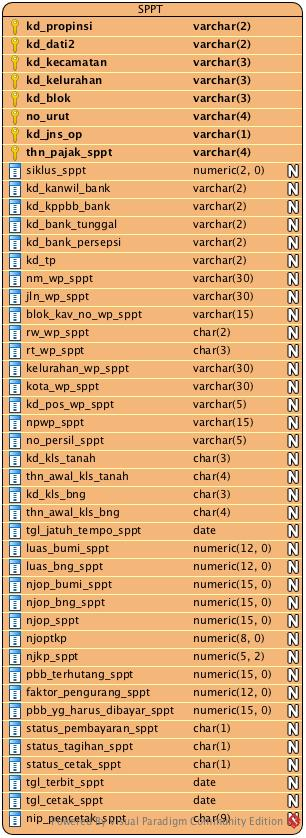
\includegraphics[width=0.5\textwidth]{./resources/struktur-tabel-sppt}
	\caption{Struktur Tabel SPPT}
	\label{fig:struktur-tabel-sppt}
\end{figure}

Penekanan pada tabel ini hanya ada pada beberapa \textit{field} atau kolom saja, yaitu pada \textit{field} atau kolom berikut :

\begin{itemize}
	\item Nomor Objek Pajak, yang terdiri dari \textit{field} atau kolom \texttt{kd\_propinsi}, \texttt{kd\_dati2}, \texttt{kd\_kecamatan}, \texttt{kd\_kelurahan}, \texttt{kd\_blok}, \texttt{no\_urut}, dan \texttt{kd\_jns\_op}.
	\item Tahun pajak pada \textit{field} atau kolom \texttt{thn\_pajak\_sppt}.
	\item Nama wajib pajak pada \textit{field} atau kolom \texttt{nm\_wp\_sppt}
	\item Besarnya pajak terhutang pada \textit{field} atau kolom \texttt{pbb\_yg\_harus\_dibayar\_sppt}
	\item Status pembayaran pada \textit{field} atau kolom \texttt{status\_pembayaran\_sppt}
\end{itemize}

\section{Tabel DAT\_OBJEK\_PAJAK}

Tabel \texttt{DAT\_OBJEK\_PAJAK}, digunakan untuk menampilkan informasi mengenai objek pajak seperti alamat, luas bumi dan bangunan, serta Nilai Jual Objek Bumi dan Bangunan. Struktur tabel dari \texttt{DAT\_OBJEK\_PAJAK} adalah seperti pada gambar \ref{fig:struktur-tabel-dat-op} berikut ini :

\begin{figure}[H]
	\centering
	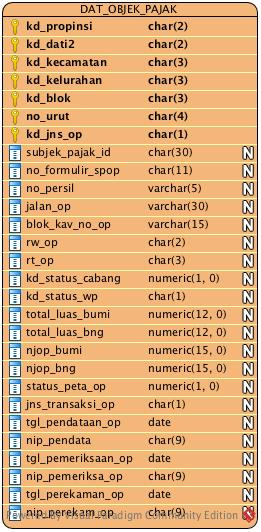
\includegraphics[width=0.5\textwidth]{./resources/struktur-tabel-dat-op}
	\caption{Struktur Tabel \texttt{DAT\_OBJEK\_PAJAK}}
	\label{fig:struktur-tabel-dat-op}
\end{figure}

\section{Tabel DAT\_SUBJEK\_PAJAK}

Tabel \texttt{DAT\_SUBJEK\_PAJAK} ini digunakan untuk menampilkan informasi mengenai subjek pajaknya seperti nama dan alamatnya. Struktur tabel dari \texttt{DAT\_SUBJEK\_PAJAK} ini adalah seperti pada gambar \ref{fig:struktur-tabel-dat-sp} berikut ini :

\begin{figure}[H]
	\centering
	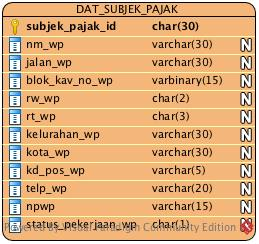
\includegraphics[width=0.5\textwidth]{./resources/struktur-tabel-dat-sp}
	\label{fig:struktur-tabel-dat-sp}
	\caption{Struktur Tabel \texttt{DAT\_SUBJEK\_PAJAK}}
\end{figure}

\section{Tabel REF\_KECAMATAN}

Untuk tabel \texttt{REF\_KECAMATAN} digunakan hanya untuk menampilkan informasi nama Kecamatan dimana objek berada. Struktur tabel untuk \texttt{REF\_KECAMATAN} ini seperti terlihat pada gambar \ref{fig:struktur-tabel-ref-kec} berikut ini :

\begin{figure}[H]
	\centering
	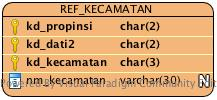
\includegraphics[width=0.5\textwidth]{./resources/struktur-tabel-ref-kec}
	\label{fig:struktur-tabel-ref-kec}
	\caption{Struktur Tabel \texttt{REF\_KECAMATAN}}
\end{figure}

\section{Tabel REF\_KELURAHAN}

Tabel \texttt{REF\_KELURAHAN} pun digunakan hanya untuk menampilkan nama Kelurahan/Desa dimana objek pajak berada. Struktur tabel \texttt{REF\_KELURAHAN} ini seperti terlihat pada gambar \ref{fig:struktur-tabel-ref-kel} berikut ini :

\begin{figure}[H]
	\centering
	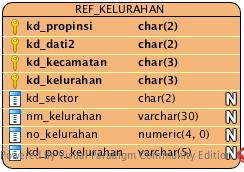
\includegraphics[width=0.5\textwidth]{./resources/struktur-tabel-ref-kel}
	\label{fig:struktur-tabel-ref-kel}
	\caption{Struktur Tabel \texttt{REF\_KELURAHAN}}
\end{figure}
\chapter{RELASI \textit{ENTITY}}

Dari tabel-tabel yang terbentuk pada bagian sebelumnya, dalam sistem ini akan membentuk sebuah jaringan relasi antar tabel dengan bentuk seperti pada gambar \ref{fig:diagram-relasi} berikut ini :

\begin{figure}[H]
	\centering
	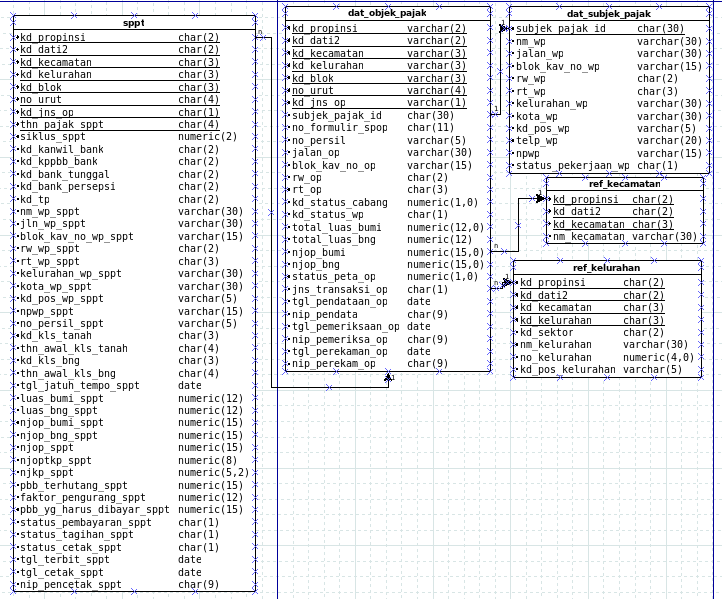
\includegraphics[width=1\textwidth]{./resources/db-diagram}
	\label{fig:diagram-relasi}
	\caption{Diagram Relasi \textit{Entity}}
\end{figure}

Titik utama akses aplikasi ini ada pada tabel \texttt{SPPT}, dimana nantinya tiap data pada tabel ini akan memiliki relasi n:1 dengan tabel \texttt{DAT\_OBJEK\_PAJAK}, ini karena tiap objek pajak yang tercatat akan memiliki banyak data SPPT untuk tiap tahun pajak.

Setiap data pada tabel \texttt{DAT\_OBJEK\_PAJAK} akan memiliki relasi 1:1 dengan data pada tabel \texttt{DAT\_SUBJEK\_PAJAK}.

Sedangkan hubungan atau relasi antara tabel \texttt{DAT\_OBJEK\_PAJAK} dengan \texttt{REF\_KECAMATAN} dan \texttt{DAT\_OBJEK\_PAJAK} dengan \texttt{REF\_KELURAHAN} adalah n:1, dimana tiap 1 (satu) data pada tabel \texttt{REF\_KECAMATAN} atau \texttt{REF\_KELURAHAN} akan memiliki banyak objek pada tabel \texttt{DAT\_OBJEK\_PAJAK}.



\backmatter%%%%%%%%%%%%%%%%%%%%%%%%%%%%%%%%%%%%%%%%%%%%%%%%%%%%%%%
\printindex

%%%%%%%%%%%%%%%%%%%%%%%%%%%%%%%%%%%%%%%%%%%%%%%%%%%%%%%%%%%%%%%%%%%%%%

\end{document}





